\section{Diskusjon}

- Hvor i smarttelefonen er sensoren plassert? \newline 
- Hva kan gjøres forskjellig for å få mer nøyaktige resultater? - Hva kan endres til neste gang? \newline
- Hvilke svakheter ligger i målingene? \newline
- Er det noen målinger som skiller seg ut? Hvorfor? \newline
- Er det nøyaktige resultater i forhold til andre type forsøk? \newline 
- Hva har resultatene å bidra med til framtidige forsøk? \newline                                    
- Bestem aksene (koordinatsystemet) til smarttelefonen. \textbf{se figur \ref{fig:telf_akser} }\newline 
- Hva er oppløsningen til sensoren? \newline 
- Er sensoren kalibrert? \newline
- Er målingene stabile? Ser du variasjoner? Er de påvirket av temperatur, lading
osv...? \textbf{Under den ene målingen når det kjørte en bil ved siden av måleapparatet, viste målingene en liten endring i dataene sammenlignet med de andre målingene. }\newline
- Er resultatene reproduserbare etter en reboot/avstengning? \newline
- Kan omgivelsene påvirke målingene? \newline                      
- Kan du detektere lokale variasjoner? Hva kan forårsake disse variasjonene?  \newline
- Avansert: Kan du oppdage variasjoner under døgnet? \newline
- Avansert: Kan nordlys påvirke målingene? \newline

\noindent\textbf{Mulige ting som kan ha påvirket resultatene}:
\begin{itemize}
    \item Forskjellige mobiltelefoner som gir forskjellige data 
    \item biler som kjører forbi
    \item andre elektromagnetiske kilder i nærheten? 
    \item trefoten kan ha vært ustødig
    \item telefonholderen
    \item vibrasjoner i bakken               
    \item siktet til vateret, er dette nøyaktig nok?
    \item Ble mobilen lagt nøyaktig nok i forhold til vateret?
    \item Værforhold - det var delvis overskyet, ingen sol
    \item flymodus, restart - hvordan påvirket dette resultatene?

\end{itemize}



\begin{figure}
    \centering
    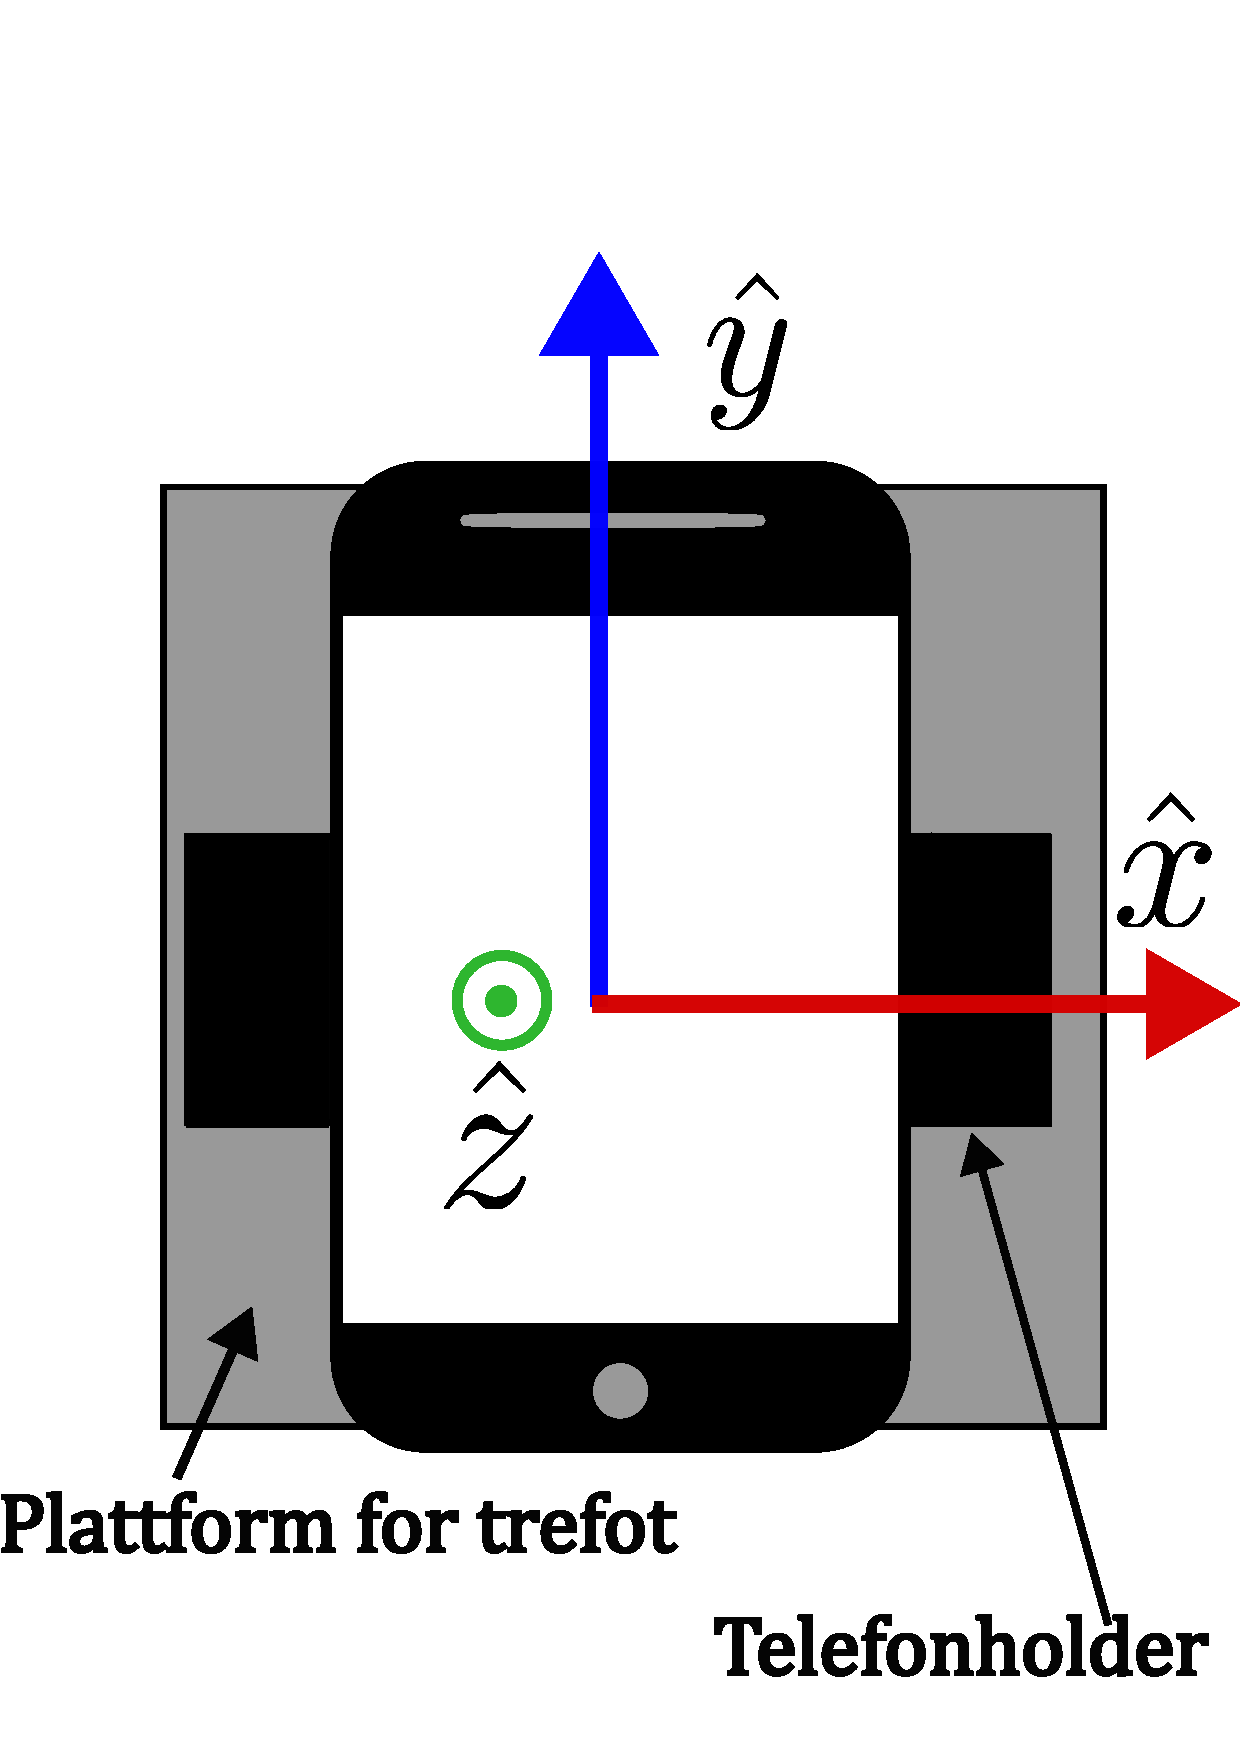
\includegraphics[width=0.65\textwidth]{img/Plattform med telefoni.pdf}
    \caption{\textbf{må kanskje endre på aksene her?} 
        }
    \label{fig:telf_akser}
\end{figure}